\clearpage
\slidetitle{Apprentissage supervisé}

\begin{slide}

\begin{itemize}

	\item Calcul de l'image $y$ par le réseau de quelques échantillons $x$.
	\begin{center}
		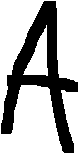
\includegraphics[width=0.075\linewidth]{a/0.png} \quad
		
\includegraphics[width=0.075\linewidth]{a/1.png} \quad
		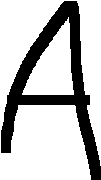
\includegraphics[width=0.075\linewidth]{a/2.png} \quad
		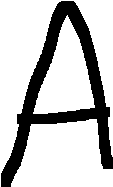
\includegraphics[width=0.075\linewidth]{a/3.png} \quad
		
\includegraphics[width=0.075\linewidth]{a/4.png}
	\end{center}
	
	\item Comparaison de $y$ et de la valeur vectorielle $t$ que l'on souhaite associer aux exemples à l'aide d'une fonction d'erreur:
	\begin{equation*}
		E = \frac{1}{2} \sum_{i=1}^q (t_i - y_i)^2.
	\end{equation*}

	\item Correction des valeurs des poids, modulée par un \textit{taux d'apprentissage} $\alpha$ que l'on fixe au départ:
	\begin{equation*}
		\Delta \poids{j}{k}{c} = - \alpha \frac{\partial E}{\partial \poids{j}{k}{c}}.
	\end{equation*}

	\item On répète ces étapes pour chaque caractère à reconnaître (associé à un unique vecteur $t$).

	\end{itemize}

\end{slide}